\documentclass[11pt, aspectratio=169]{beamer}

% LuaLaTeXで日本語を使うための必須パッケージ（英語のみの場合は外しても動きますが、そのまま残しています）
\usepackage{luatexja}

% 便利な追加パッケージ
\usepackage{booktabs}   % 表の罫線
\usepackage{tikz}       % 図形描画
\usepackage{listings}   % ソースコード挿入
\lstset{
  basicstyle=\ttfamily\scriptsize,
  frame=single,
  breaklines=true,
  numbers=left,
  numberstyle=\tiny
}

% テーマとカラーテーマの設定
\usetheme{Madrid}
\usecolortheme{orchid}

% ==========================================
% セクション・サブセクションの可視化設定
% ==========================================

% 1. セクション開始時の自動表紙（大きな扉絵）
\AtBeginSection[]{
  \begin{frame}
    \vfill
    \centering
    \begin{beamercolorbox}[sep=8pt,center,shadow=true,rounded=true]{title}
      \usebeamerfont{title}\insertsectionhead\par%
    \end{beamercolorbox}
    \vfill
  \end{frame}
}

% 2. サブセクション開始時に「現在のセクション内の目次」を自動挿入
\AtBeginSubsection[]{
  \begin{frame}{\insertsectionhead}
    \tableofcontents[currentsection, currentsubsection, subsectionstyle=show/shaded/hide]
  \end{frame}
}

% タイトル情報
\title{Overview of Jamming Communications and Future Plans}
\subtitle{Jamming Communications}
\author{Student ID: 1280391 \\ Name: Natsuka Hosokawa}
\institute{Kochi University of Technology}
\date{\today}

\begin{document}

\usetikzlibrary{decorations.pathmorphing}

% タイトルスライド
\begin{frame}
  \titlepage
\end{frame}

\begin{frame}{Progress}
  \begin{enumerate}[1]
    \item Jamming in SAGIN
    \item Overview of SAGIN
    \item Overview of Jamming (Current)
  \end{enumerate}
\end{frame}

% 全体目次スライド
\begin{frame}{Table of Contents}
  \tableofcontents
\end{frame}

% ==========================================
% ここから本文
% ==========================================

\section{What is Jamming?}
\subsection{Overview}

\begin{frame}{Overview}
  \begin{columns}[c, onlytextwidth]
    
    % --- 左側：テキスト部 ---
    \begin{column}{0.52\textwidth}
      Since wireless communication relies on a shared medium, jamming is relatively easy to execute and difficult to defend against.
    
      \vspace{1em}
    
      If the interference (noise) is too high, the receiver cannot distinguish between $1$ and $0$, making communication impossible.
    
      \vspace{1.5em}
    
      \begin{block}{Summary}
        Jamming is an attack that intentionally broadcasts high-power interference signals into a shared medium to drown out legitimate communication.
      \end{block}
    \end{column}
    
    \hfill
    
    % --- 右側：TikZ図解部 ---
    \begin{column}{0.5\textwidth}
      \centering
      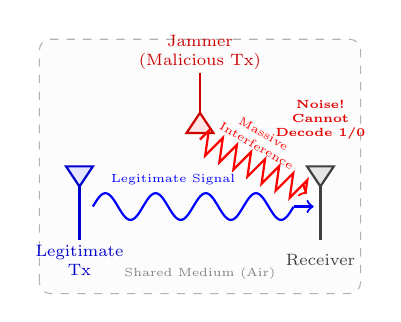
\begin{tikzpicture}[scale=0.85, transform shape]
        % 共通空間の枠
        \draw[dashed, gray!60, rounded corners, fill=gray!2] (-0.6, -1.3) rectangle (4.2, 2.5);
        \node at (1.8, -1.0) [gray, font=\tiny] {Shared Medium (Air)};

        % 1. 正規送信機（左）
        \draw[thick, blue!80!black] (0,-0.5) -- (0,0.3);
        \draw[thick, blue!80!black, fill=blue!10] (0,0.3) -- (-0.2,0.6) -- (0.2,0.6) -- cycle;
        \node at (0,-0.8) [blue!80!black, font=\scriptsize, align=center] {Legitimate\\Tx};

        % 2. 受信機（右）
        \draw[thick, darkgray] (3.6,-0.5) -- (3.6,0.3);
        \draw[thick, darkgray, fill=gray!20] (3.6,0.3) -- (3.4,0.6) -- (3.8,0.6) -- cycle;
        \node at (3.6,-0.8) [darkgray, font=\scriptsize, align=center] {Receiver};

        % 3. 妨害機（上）
        \draw[thick, red!80!black] (1.8,2.0) -- (1.8,1.4);
        \draw[thick, red!80!black, fill=red!10] (1.8,1.4) -- (1.6,1.1) -- (2.0,1.1) -- cycle;
        \node at (1.8,2.3) [red!80!black, font=\scriptsize, align=center] {Jammer\\(Malicious Tx)};

        % 4. 正規の電波（きれいなサイン波）
        \draw[blue, thick, domain=0.2:3.2, samples=100] plot (\x, {0.2*sin((\x-0.2)/3.0 * 4 * 360)});
        \draw[blue, thick, ->] (3.2,0) -- (3.5,0);
        \node at (1.4, 0.4) [blue, font=\tiny] {Legitimate Signal};

        % 5. 妨害電波（ギザギザのノイズ波）
        \draw[red, thick, ->, decorate, decoration={zigzag, amplitude=1.5mm, segment length=2mm}] (1.8, 1.0) -- (3.4, 0.2);
        \node at (2.7, 1.0) [red, font=\tiny, align=center, rotate=-30] {Massive\\Interference};

        % 6. 受信機での混信状態のラベル
        \node at (3.6, 1.3) [red!90!black, font=\bfseries\tiny, align=center] {Noise!\\Cannot\\Decode 1/0};
      \end{tikzpicture}
    \end{column}
    
  \end{columns}
\end{frame}

\subsection{Types of Jamming}

\begin{frame}{Types of Jamming}
  \begin{columns}[c, onlytextwidth]
    
    % --- 左側：テキスト部 ---
    \begin{column}{0.5\textwidth}
      \begin{itemize}
        \item \textbf{Continuous Jamming}:\\
          Continuously emits high-power interference signals.

          \vspace{1em}

          \alert{Very effective at disrupting communication, but rapidly depletes the attacker's battery.}
      \end{itemize}
    \end{column}
    
    \hfill
    
    % --- 右側：TikZ図解部 ---
    \begin{column}{0.45\textwidth}
      \centering
      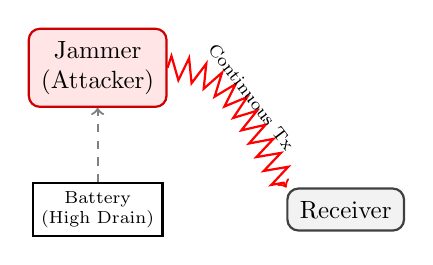
\begin{tikzpicture}[scale=0.9, transform shape]
        % 妨害機
        \node[draw=red!80!black, thick, fill=red!10, rounded corners, align=center, inner sep=5pt] (attacker) at (0, 2) {Jammer\\(Attacker)};
        
        % 受信機
        \node[draw=darkgray, thick, fill=gray!10, rounded corners, align=center, inner sep=5pt] (receiver) at (3.5, 0) {Receiver};
        
        % バッテリー
        \node[draw=black, thick, fill=white, align=center, font=\scriptsize] (battery) at (0, 0) {Battery\\(High Drain)};
        
        % バッテリーから妨害機への線
        \draw[->, thick, gray, dashed] (battery.north) -- (attacker.south);
        
        % 妨害電波の矢印
        \draw[->, red, thick, decorate, decoration={zigzag, amplitude=1.5mm, segment length=2mm}] 
          (attacker.east) to[out=0, in=120] node[above, sloped, font=\scriptsize, text=black] {Continuous Tx} (receiver.north west);
      \end{tikzpicture}
    \end{column}
    
  \end{columns}
\end{frame}

\begin{frame}{Types of Jamming}
  \begin{columns}[c, onlytextwidth]
    
    % --- 左側：テキスト部 ---
    \begin{column}{0.52\textwidth}
      \begin{itemize}
        \item \textbf{Reactive Jamming}: \\
          Remains idle normally, but transmits an interference signal the moment legitimate communication is detected.

        \vspace{1em}

        \alert{Highly energy-efficient and difficult to detect since it only operates when necessary.}
      \end{itemize}
    \end{column}
    
    \hfill
    
    % --- 右側：TikZ図解部 ---
    \begin{column}{0.45\textwidth}
      \centering
      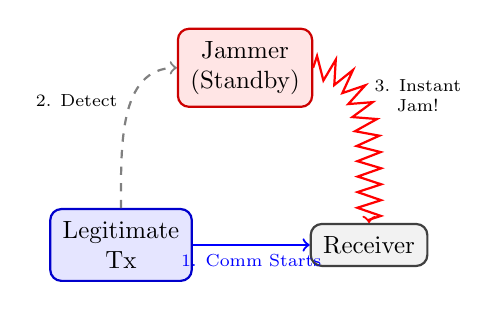
\begin{tikzpicture}[scale=0.9, transform shape]
        % 正規送信機
        \node[draw=blue!80!black, thick, fill=blue!10, rounded corners, align=center, inner sep=5pt] (sender) at (0, 0) {Legitimate\\Tx};
        
        % 受信機
        \node[draw=darkgray, thick, fill=gray!10, rounded corners, align=center, inner sep=5pt] (receiver) at (3.5, 0) {Receiver};
        
        % 妨害機
        \node[draw=red!80!black, thick, fill=red!10, rounded corners, align=center, inner sep=5pt] (attacker) at (1.75, 2.5) {Jammer\\(Standby)};
        
        % 1. 正規の通信
        \draw[->, thick, blue] (sender.east) -- node[below, font=\scriptsize] {1. Comm Starts} (receiver.west);
        
        % 2. 通信の検知
        \draw[->, thick, gray, dashed] (sender.north) to[out=90, in=180] node[above left, font=\scriptsize, text=black] {2. Detect} (attacker.west);
        
        % 3. 妨害電波
        \draw[->, red, thick, decorate, decoration={zigzag, amplitude=1.5mm, segment length=2mm}] 
          (attacker.east) to[out=0, in=90] node[above right, font=\scriptsize, text=black, align=center] {3. Instant\\Jam!} (receiver.north);
      \end{tikzpicture}
    \end{column}
  \end{columns}
\end{frame}

\begin{frame}{Types of Jamming}
  \begin{columns}[c]
    
    % --- 左側：テキスト部分（幅55%） ---
    \begin{column}{0.55\textwidth}
      \begin{itemize}
        \item \textbf{Smart Jamming}: \\
          Rather than jamming all data, it targets critical control packets or synchronization signals required to establish a connection.
          
          \vspace{1em}
          \alert{Commonly used against \texttt{Wi-Fi} and $5$\texttt{G} networks.}
      \end{itemize}
    \end{column}
    
    % --- 右側：図の部分（幅45%） ---
    \begin{column}{0.45\textwidth}
      \centering
      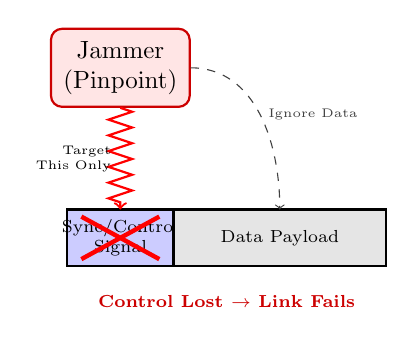
\begin{tikzpicture}[scale=0.9, transform shape]
        % パケット全体の描画
        % 1. 同期/制御信号のブロック（攻撃対象）
        \draw[thick, fill=blue!20] (0, 0) rectangle (1.5, 0.8);
        \node at (0.75, 0.4) [font=\scriptsize, align=center] {Sync/Control\\Signal};
        
        % 2. データ本体のブロック
        \draw[thick, fill=gray!20] (1.5, 0) rectangle (4.5, 0.8);
        \node at (3.0, 0.4) [font=\scriptsize] {Data Payload};
        
        % 妨害機
        \node[draw=red!80!black, thick, fill=red!10, rounded corners, align=center, inner sep=5pt] (attacker) at (0.75, 2.8) {Jammer\\(Pinpoint)};
        
        % 妨害電波（制御信号のみを狙う）
        \draw[->, red, thick, decorate, decoration={zigzag, amplitude=1.5mm, segment length=2mm}] 
          (attacker.south) -- node[left, font=\tiny, text=black, align=right] {Target\\This Only} (0.75, 0.8);
        
        % データはスルーしていることを示す線
        \draw[->, darkgray, dashed] (attacker.east) to[out=0, in=90] node[right, font=\tiny, text=darkgray] {Ignore Data} (3.0, 0.8);
        
        % 破壊エフェクト（バツ印）
        \draw[ultra thick, red] (0.2, 0.1) -- (1.3, 0.7);
        \draw[ultra thick, red] (0.2, 0.7) -- (1.3, 0.1);
        
        % 結果の注釈
        \node at (2.25, -0.5) [font=\scriptsize\bfseries, red!80!black] {Control Lost $\rightarrow$ Link Fails};
      \end{tikzpicture}
    \end{column}
    
  \end{columns}
\end{frame}

\subsection{Summary}

\begin{frame}{Summary}
  \begin{block}{}
    As outlined above, there are various types of jamming attacks, each with distinct advantages, disadvantages, and specific use cases depending on the scenario.
  \end{block}
\end{frame}

\section{Anti-Jamming Countermeasures}

\subsection{Common Countermeasures}

\begin{frame}{Common Countermeasures}
  \begin{columns}[c]
    
    % --- 左側：テキスト部分（幅55%） ---
    \begin{column}{0.55\textwidth}
      \begin{itemize}
        \item \textbf{Frequency Hopping}: \\
          Rapidly switches the carrier frequency during transmission based on a predetermined pseudorandom sequence.
        
          \vspace{1.5em}
    
        \alert{Makes it extremely difficult for an attacker to predict and jam the active frequency band. Widely used in \texttt{Bluetooth}.}
      \end{itemize}
    \end{column}
    
    % --- 右側：図の部分（幅45%） ---
    \begin{column}{0.45\textwidth}
      \centering
      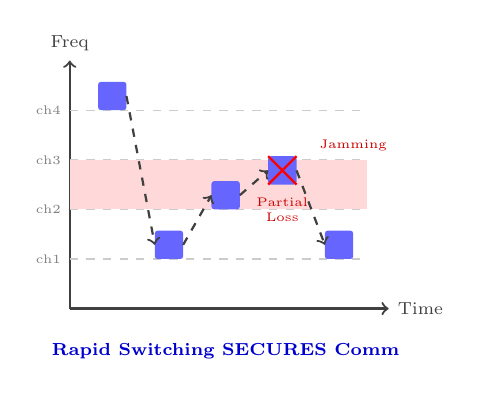
\begin{tikzpicture}[scale=0.9, transform shape]
        % 軸の描画
        \draw[->, thick, darkgray] (0,0) -- (4.5,0) node[right, font=\scriptsize] {Time};
        \draw[->, thick, darkgray] (0,0) -- (0,3.5) node[above, font=\scriptsize] {Freq};
        
        % チャンネルの補助線
        \foreach \y in {1,2,3,4} {
          \draw[dashed, gray!40] (0,\y*0.7) -- (4.2,\y*0.7);
          \node[left, font=\tiny, text=gray] at (0,\y*0.7) {ch\y};
        }
        
        % 攻撃者による妨害電波
        \fill[red!15] (0, 1.4) rectangle (4.2, 2.1);
        \node[red!80!black, font=\tiny, align=left] at (4.0, 2.3) {Jamming};
        
        % ホッピングする通信データ
        \fill[blue!60, rounded corners=1pt] (0.4, 2.8) rectangle (0.8, 3.2); 
        \fill[blue!60, rounded corners=1pt] (1.2, 0.7) rectangle (1.6, 1.1); 
        \fill[blue!60, rounded corners=1pt] (2.0, 1.4) rectangle (2.4, 1.8); 
        
        % 妨害と衝突するデータ
        \fill[blue!60, rounded corners=1pt] (2.8, 1.75) rectangle (3.2, 2.15); 
        \draw[thick, red] (2.8, 1.75) -- (3.2, 2.15); 
        \draw[thick, red] (2.8, 2.15) -- (3.2, 1.75);
        
        \fill[blue!60, rounded corners=1pt] (3.6, 0.7) rectangle (4.0, 1.1); 
        
        % ホッピングの軌跡
        \draw[->, thick, darkgray, dashed] (0.8, 3.0) -- (1.2, 0.9);
        \draw[->, thick, darkgray, dashed] (1.6, 0.9) -- (2.0, 1.6);
        \draw[->, thick, darkgray, dashed] (2.4, 1.6) -- (2.8, 1.95);
        \draw[->, thick, darkgray, dashed] (3.2, 1.95) -- (3.6, 0.9);
        
        % 注釈
        \node[font=\scriptsize\bfseries, blue!80!black] at (2.2, -0.6) {Rapid Switching SECURES Comm};
        \node[font=\tiny, red!80!black, align=center] at (3.0, 1.4) {Partial\\Loss};
      \end{tikzpicture}
    \end{column}
  \end{columns}
\end{frame}

\begin{frame}{Common Countermeasures}
  \begin{columns}[c]
    
    % --- 左側：テキスト部分（幅53%） ---
    \begin{column}{0.53\textwidth}
      \begin{itemize}
        \item \textbf{Spread Spectrum}: \\
          A method that spreads the transmitted signal over a much wider frequency band than originally required.
        
          \vspace{1.5em}
    
        \alert{Highly resilient to noise. When the receiver despreads the signal, the jammer's power is diluted across the wideband, neutralizing the attack.}
      \end{itemize}
    \end{column}
    
    % --- 右側：図の部分（幅47%） ---
    \begin{column}{0.47\textwidth}
      \centering
      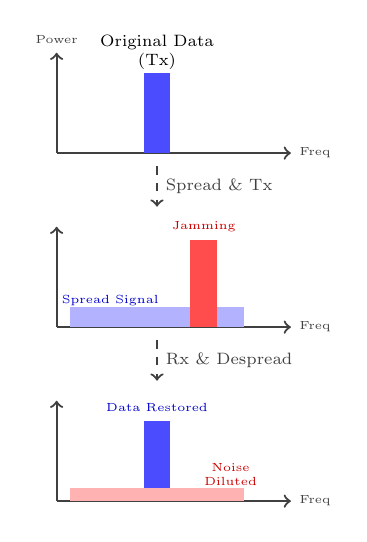
\begin{tikzpicture}[scale=0.85, transform shape]
        % 1. 送信時のデータ
        \draw[->, thick, darkgray] (0, 0) -- (3.5, 0) node[right, font=\tiny] {Freq};
        \draw[->, thick, darkgray] (0, 0) -- (0, 1.5) node[above, font=\tiny] {Power};
        \fill[blue!70] (1.3, 0) rectangle (1.7, 1.2);
        \node[font=\scriptsize, align=center] at (1.5, 1.5) {Original Data\\(Tx)};
        
        % 拡散の矢印
        \draw[->, thick, darkgray, dashed] (1.5, -0.2) -- (1.5, -0.8) node[midway, right, font=\scriptsize] {Spread \& Tx};
        
        % 2. 空間での状態
        \begin{scope}[yshift=-2.6cm]
          \draw[->, thick, darkgray] (0, 0) -- (3.5, 0) node[right, font=\tiny] {Freq};
          \draw[->, thick, darkgray] (0, 0) -- (0, 1.5);
          \fill[blue!30] (0.2, 0) rectangle (2.8, 0.3);
          \node[font=\tiny, text=blue!80!black] at (0.8, 0.4) {Spread Signal};
          \fill[red!70] (2.0, 0) rectangle (2.4, 1.3);
          \node[font=\tiny, text=red!80!black] at (2.2, 1.5) {Jamming};
        \end{scope}
        
        % 逆拡散の矢印
        \draw[->, thick, darkgray, dashed] (1.5, -2.8) -- (1.5, -3.4) node[midway, right, font=\scriptsize] {Rx \& Despread};
        
        % 3. 受信時の状態
        \begin{scope}[yshift=-5.2cm]
          \draw[->, thick, darkgray] (0, 0) -- (3.5, 0) node[right, font=\tiny] {Freq};
          \draw[->, thick, darkgray] (0, 0) -- (0, 1.5);
          \fill[blue!70] (1.3, 0) rectangle (1.7, 1.2);
          \node[font=\tiny, text=blue!80!black] at (1.5, 1.4) {Data Restored};
          \fill[red!30] (0.2, 0) rectangle (2.8, 0.2);
          \node[font=\tiny, text=red!80!black, align=center] at (2.6, 0.4) {Noise\\Diluted};
        \end{scope}
      \end{tikzpicture}
    \end{column}
  \end{columns}
\end{frame}

\begin{frame}{Common Countermeasures}
  \begin{columns}[c]
    
    % --- 左側：テキスト部分（幅55%） ---
    \begin{column}{0.55\textwidth}
      \begin{itemize}
        \item \textbf{\texttt{MIMO} and Spatial Filtering}: \\
          Utilizes multiple antennas at both the base station and the user equipment.
    
        \vspace{1em}
    
        By leveraging multiple antennas, the receiver can \alert{calculate the Direction of Arrival (DoA) of both the legitimate signal and the jamming signal}. The receiver can then create a spatial "null" to physically block the interference.
      \end{itemize}
    \end{column}
    
    % --- 右側：図の部分（幅45%） ---
    \begin{column}{0.45\textwidth}
      \centering
      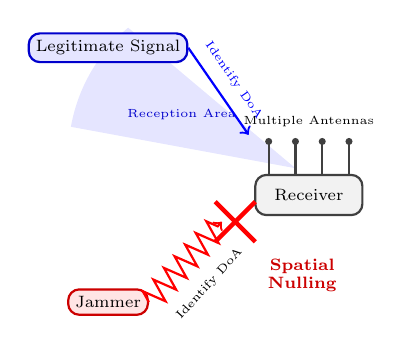
\begin{tikzpicture}[scale=0.85, transform shape]
        % 受信エリア
        \fill[blue!10] (2.3, 0.4) -- (-0.2, 2.5) arc (130:170:2.5) -- cycle;
        \node[font=\tiny, text=blue!80!black] at (0.6, 1.2) {Reception Area};

        % 受信機
        \node[draw=darkgray, thick, fill=gray!10, rounded corners, minimum width=1.6cm, minimum height=0.6cm, align=center, font=\scriptsize] (rx) at (2.5, 0) {Receiver};
        
        % アンテナ素子
        \foreach \x in {1.9, 2.3, 2.7, 3.1} {
            \draw[thick, darkgray] (\x, 0.3) -- (\x, 0.8);
            \fill[darkgray] (\x, 0.8) circle (1.5pt);
        }
        \node[font=\tiny] at (2.5, 1.1) {Multiple Antennas};

        % 1. 正規の通信
        \node[draw=blue!80!black, thick, fill=blue!10, rounded corners, inner sep=3pt, font=\scriptsize] (tx) at (-0.5, 2.2) {Legitimate Signal};
        \draw[->, thick, blue] (tx.east) -- node[above, sloped, font=\tiny, yshift=2pt] {Identify DoA} (1.6, 0.9);

        % 2. 妨害機
        \node[draw=red!80!black, thick, fill=red!10, rounded corners, inner sep=3pt, font=\scriptsize] (jammer) at (-0.5, -1.6) {Jammer};
        
        \draw[->, thick, red, decorate, decoration={zigzag, amplitude=1.5mm, segment length=2mm}] 
          (jammer.east) -- node[below, sloped, font=\tiny, text=black, yshift=-8pt] {Identify DoA} (1.2, -0.4);

        % バツ印
        \draw[ultra thick, red] (1.1, -0.1) -- (1.7, -0.7);
        \draw[ultra thick, red] (1.1, -0.7) -- (1.7, -0.1);
        \node[font=\scriptsize\bfseries, text=red!80!black, align=center] at (2.4, -1.2) {Spatial\\Nulling};
      \end{tikzpicture}
    \end{column}
    
  \end{columns}
\end{frame}

\subsection{Counter-Countermeasures}

\begin{frame}{The Nature of Security}
  \begin{block}{An Endless Cat-and-Mouse Game}
    Naturally, these countermeasures do not provide perfect protection. Attackers continuously develop advanced methods (counter-countermeasures) to bypass these defenses. This evolutionary arms race is the fundamental nature of cybersecurity. While it is a complex field, I plan to delve into these advanced adversarial dynamics in my future studies.
  \end{block}
\end{frame}

\subsection{Summary}

\begin{frame}{Summary}
  \begin{block}{}
    While various anti-jamming techniques exist, none offer a universal shield against all attack vectors. It is crucial to understand how defenses are implemented, how attackers attempt to circumvent them, and to continually devise robust, next-generation countermeasures.
  \end{block}
\end{frame}

\section{Current Progress and Future Plans}

\subsection{Planned Simulation Environment}

\begin{frame}{Simulation Environment}
  Setup for Jamming Communications Simulation
  \begin{itemize}
    \item Server Environment (TBD): \\
      However, \texttt{Dockerfile} and \texttt{docker-compose.yaml} have already been created, enabling immediate deployment.
    \item Required Library (\textbf{\texttt{PyJama}}): 
      \begin{itemize}
        \item Expected to run on \texttt{Python 3.10-slim}.
        \item Assumes the use of a \texttt{GPU} to accelerate matrix operations and tensor calculations.
        \item Available as \texttt{OSS} on GitHub: \texttt{https://github.com/IIP-Group/pyjama}
      \end{itemize}
  \end{itemize}
\end{frame}

\subsection{Future Study Plans}

\begin{frame}{Future Study Plans}
  \begin{itemize}
    \item Study the underlying mathematics and mechanisms of signal jamming.
    \item Study Reinforcement Learning (RL) in Prof. Wei's seminar.
    \item Study Game Theory to predict optimal jamming and defense strategies, which will be integrated with RL models.

    \vspace{1em}

    \item Develop a simplified \texttt{Python} program to simulate basic jamming attacks.
  \end{itemize}
\end{frame}

\section{References}

\begin{frame}[allowframebreaks]{References}
  \begin{thebibliography}{9}
    
    % Comprehensive survey paper used as the base (covering jamming techniques and countermeasures)
    \bibitem{Pirayesh2022}
    Hossein Pirayesh and Huacheng Zeng.
    \newblock Jamming Attacks and Anti-Jamming Strategies in Wireless Networks: A Comprehensive Survey.
    \newblock \emph{IEEE Communications Surveys \& Tutorials}, 2022.

    % Paper on jamming against OFDM systems and mathematical defense strategies
    \bibitem{Yun202X}
    Jaewon Yun, Joohyuk Park, and Yo-Seb Jeon.
    \newblock Anti-Jamming Modulation for OFDM Systems under Jamming Attacks.
    \newblock \emph{arXiv preprint arXiv:2510.02640}.

    % Recent survey on security threats and countermeasures in the 5G physical layer
    \bibitem{Harvanek2024}
    Michal Harvanek, et al.
    \newblock Survey on 5G Physical Layer Security Threats and Countermeasures.
    \newblock \emph{Sensors}, 2024.
      
    % Document on next-generation electronic warfare using AI and networks
    \bibitem{Amagai2020}
    Takaki Amagai.
    \newblock On Next-Generation Electronic Warfare: EMS Operations Utilizing Machine Learning and Networks.
    \newblock \emph{Strategic Studies of JMSDF Staff College}, 2020.

  \end{thebibliography}
\end{frame}

\end{document}